
La técnica de la reacción en cadena de la polimerasa, o PCR por sus siglas en inglés, (Polymerase Chain Reaction) es una técnica de biología molecular desarrollada en 1983 por Kary Mullis.

Su objetivo es, a partir de una mínima cantidad de ADN, obtener un gran número de copias de un fragmento de ADN particular; en teoría basta partir de una sola copia de ese fragmento original, o molde, para crea una gran cantidad de copias del mismo.

\section{Conceptos básicos de la PCR}

\subsection{Clásica o punto final}

Este método consiste unicamente en los pasos básicos de la PCR (Desnaturalización, alineación y elongación). Tiene la desventaja de necesitar un proceso posterior (electroforesis en gel) para poder cuantificar la cantidad de ADN obtenido. 

\begin{figure}[H]
    \centering
    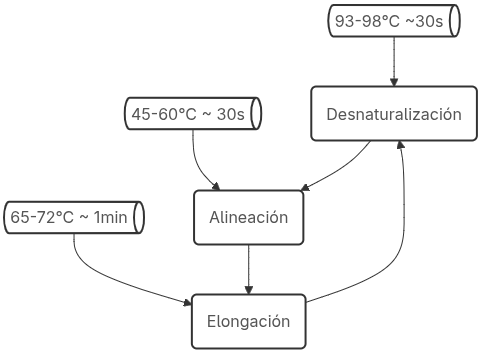
\includegraphics[width=0.65\linewidth]{images/09_pcr-method.png}
    \caption{Metodología de la PCR clásica}
    \label{fig:pcr-method}
\end{figure}


\section{Reactivos, materiales y equipos utilizados para la PCR}

Si bien los reactivos necesarios para llevar acabo una una PCR pueden variar dependiendo de la metodología usada,  podemos enlistar los elementos más usados de la siguiente manera:

\begin{itemize}
    \item Buffer
    \item Muestra de ADN o ARN
    \item Enzima polimerasa (Taq-polimerasa)
    \item Cofactor de la polimerasa
    \item Primers
    \item dNTP's
    \item Agua
    \item Enzima RT (en ocasiones)
\end{itemize}

\subsection{Reactivos}

\subsubsection{Buffer}
Se utiliza para mantener las muestras estables.

\subsubsection{Muestra de ADN o ADNc (complementario)}

Es la muestra que se desea amplificar.

\subsubsection{Enzima polimerasa}

Es la protagonista de la reacción. Elonga las secciones de interés de la muestra de ADN proporcionada. Puesto que los procesos de la PCR necesitan de cambios de la temperatura, llegando incluso hasta 98°C, el usar polimerasas comunes no es viable, pues sería necesario agregar la enzima cada vez que la temperatura suba, lo que aumentaría los costos del proceso, el tiempo que tomaría realizarlo y su dificultad.

En 1964, Thomas D. Brock y Hudson Freezen descubrieron un organismo termófilo en las aguas termales de Yellowstone, y lo llamaron \textit{Thermus aquaticus}. En 1980, Kary Mullis, trabajando para Cetus Corporation, utilizó la polimerasa de este organismo para el nuevo procedimiento que estaba desarrollando, la PCR. Esta enzima, llamada Taq-polimerasa, podía soportar las altas temperaturas necesarias en la PCR gracias a las características del organismo de donde se aisló.

\subsubsection{Cofactor de polimerasa}

La enzima polimerasa necesita de un cofactor para poder realizar su función. El cofactor más utilizado es el \textbf{cloruro de magnesio (MgCl2)}.

\subsubsection{Primers}

Son fragmentos de ADN que se unen a las cadenas de ADN, esto con el objetivo de indicarle a la polimerasa el punto de inicio para llevar a cabo la elongación.
Estos primers suelen tener un tamaño de entre 10 y 15 pares de bases.

\subsubsection{dNTP's}

Son nucleotidos "sueltos" agregados al medio con los cuales la polimerasa puede trabajar y sintetizar ADN.

\subsubsection{Agua}

Generalmente se recomienda el uso de agua con cierta calidad de pureza, como el agua tratada con DEPC (di-etil-pirocarbonato), o el agua libre de nucleasas.

\subsubsection{Enzima RT (Retrotranscriptasa o transcriptasa-inversa)}

La polimerasa usada en la PCR trabaja con ADN, por lo que de querer analizar muestras de ARN (por ejemplo, muestras de virus) se necesita transformar el ARN en ADN. Para esto se usa una enzima llamada retrotranscriptasa o transcriptasa inversa, también abreviada como enzima RT.

Esta enzima convierte ARN's en ADN complementario (ADNc), y se usa previo a la PCR añadiendo las enzimas RT y temperatura, usualmente de entre 45-50°C durante 30 minutos, aunque las temperaturas y tiempos exactos van a variar dependiendo el contexto.

Una RT ampliamente usada es la MMLV-RT (Moloney Murine Leukemia Virus - Retro-Transcriptase), aislada del virus de la leucemia murina de Moloney.

\subsection{Materiales}

Los materiales necesarios para realizar una PCR suelen ser pocos:

\begin{itemize}
    \item Micropipetas
    \item Tubos eppendorf (de entre 1.5ml y 0.2ml)
    \item Tubos o placas ópticas de 0.2ml
\end{itemize}

\subsection{Equipos}

Respecto a los equipos, al igual que los materiales, suelen ser pocos y siempre los mismso los que se usan para realizar una PCR

\begin{itemize}
    \item Termociclador: Es el equipo encargado de manejar los cambios de temperatura necesarios para que ocurra la PCR. Existen varios tipos de termocicladores.
        \begin{itemize}
            \item Clásico
            \item Tiempo real
            \item Digital
        \end{itemize}
    
    \item Centrífuga: Es utilizada para separar fases de la muestra.  
\end{itemize}

\section{Enzimas de restricción}



\section{Ciclos de la PCR}

La PCR funciona subiendo y bajando la temperatura de las muestras de ADN, esto para que ocurran las diferentes reacciones que permiten la generación de copias de ADN. Esto se compone de \textbf{3 pasos} que se repiten una y otra vez, y es lo que se conoce como \textbf{ciclo}.

\begin{figure}[H]
    \centering
    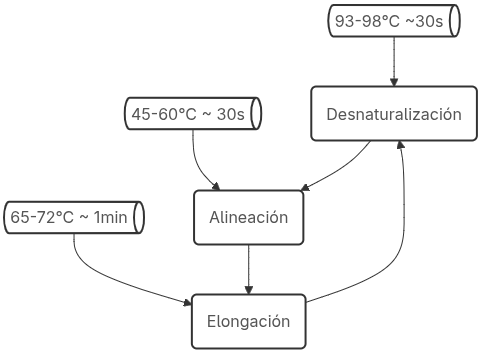
\includegraphics[width=0.65\linewidth]{images/09_pcr-method.png}
    \caption{Metodología básica de una PCR}
    \label{fig:pcr-method}
\end{figure}

\subsection{Desnaturalización}

En este primer paso, se aumenta la temperatura de la muestra de ADN, esto para hacer que la doble hélice se separe y que las hebras estén "disponibles" para que la polimerasa pueda realizar  su trabajo (elongar).

La temperatura a la que se lleva suele estar \textbf{entre 93 y 98°C}, usualmente usandose el punto medio, 95°C. Esta temperatura se mantiene durante, aproximadamente \textbf{30 segundos}.

\subsection{Alineación}

Una vez separadas las cadenas de ADN, los primers se unen al sector para el que fueron diseñados, esto para que la polimerasa pueda tener un sector desde el cual iniciar.

Para este paso la temperatura se reduce hasta \textbf{45-60°C}, y se mantiene así aproximadamente \textbf{30 segundos}.

\subsection{Elongación}

Una vez separadas las hebras de ADN y que los primers se hubieran unido a este ADN, la polimerasa puede elongar los sectores de interés.

Aquí se vuelve a aumentar la temperatura hasta \textbf{65-72°C} durante \textbf{1 minuto}.

\section{Variantes de la PCR}

Existen diferentes formas de realizar la PCR, sin embargo, el proceso de la PCR descrito anteriormente suele variar poco entre estos métodos. Los tipos de PCR principales son:

\begin{itemize}
    \item Tiempo real (qPCR)
    \item Retrotranscriptasa (RT-PCR)
    \item Combinación Retrotranscriptasa-Tiempo Real (RT-qPCR)
    \item Digital
\end{itemize}

\subsection{Tiempo real (qPCR)}

Este también sigue los pasos anteriormente descritos, pero hace uso de termocicladores que miden la cantidad de ADN generado al mismo tiempo que llevan el proceso de PCR.
Esto se logra agregando sustancias que pueden ser medidas mediante espectrofotometría, y después de cada ciclo el termociclador toma una medición de estas sustancias mediante el uso de \textbf{luz UV}.

Este proceso necesita de material de referencia y da como resultado una gráfica que usualmente se ve como una \textbf{curva sigmoide}, cuyo eje x mide los ciclos que pasan y el eje y es la absorbancia.

\begin{figure}[H]
    \centering
    \begin{subfigure}{0.4\textwidth}
        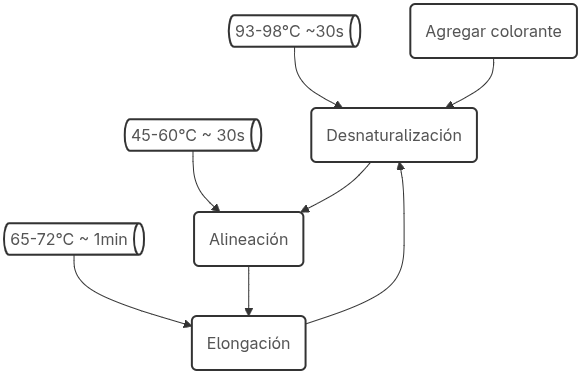
\includegraphics[width=\linewidth]{images/09_qpcr-method.png}
        \caption{Metodología de una PCR en tiempo real (qPCR)}
        \label{fig:qpcr-method}
    \end{subfigure}
    \hspace{0.1\textwidth}
    \begin{subfigure}{0.4\textwidth}
        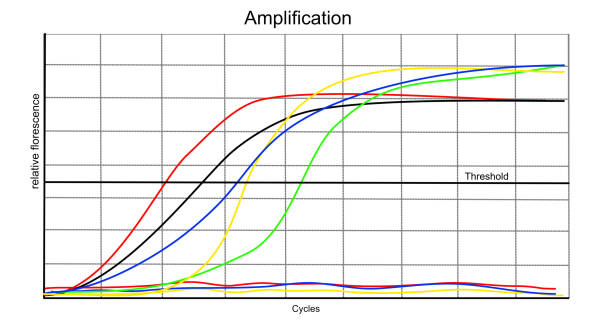
\includegraphics[width=\linewidth]{images/09_qpcr-graph.jpg}
        \caption{Ejemplo de gráfica resultante de una qPCR}
        \label{fig:qpcr-graph}
    \end{subfigure}
    
    \caption{Metodología y resultados de una qPCR}
    \label{fig:qpcr-images}
\end{figure}

\subsection{RT-PCR (Retrotranscriptasa-PCR)}

Este, más que un método de PCR, es un paso que se realiza previo a la PCR.
Cuando se cuenta con muestras de ARN, es necesario convertirlas a ADN, por lo que se utiliza la \textbf{enzima RT} (retro-transcriptasa) para realizar tal conversión. Una vez realizado esto, se puede proseguir con la técnica de PCR que se desee.

\begin{figure}[H]
    \centering
    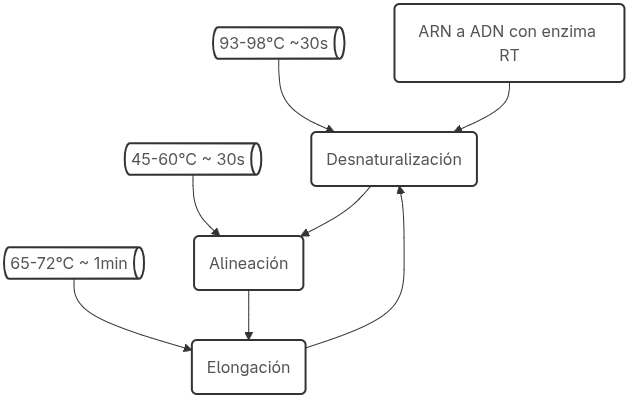
\includegraphics[width=0.65\linewidth]{images/09_rt-pcr-method.png}
    \caption{Metodología de una RT-PCR}
    \label{fig:rt-pcr-method}
\end{figure}

\subsection{RT-qPCR}

Se abrevia así cuando se realizan el proceso de RT-PCR seguido de una qPCR.

\begin{figure}[H]
    \centering
    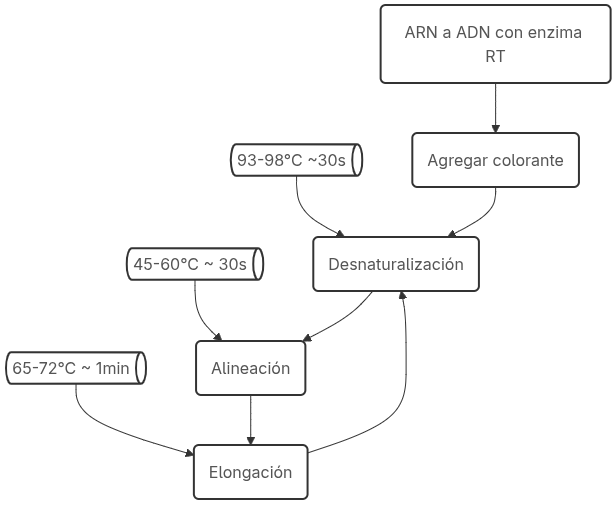
\includegraphics[width=0.65\linewidth]{images/09_rt-qpcr-method.png}
    \caption{Metodología de una RT-qPCR}
    \label{fig:rt-qpcr-method}
\end{figure}

\subsection{Digital}

En este método, el proceso está casi completamente automatizado mendiante el uso de máquinas especializadas.

\section{Analisis de datos de PCR's}

Una vez se realiza una PCR, la muestra y/o datos obtenidos se analizan para determinar diferentes aspectos de la muestra (cantidad de ADN generado, diferenciación entre genes generados, etcétera)

\subsection{Clasica o punto final}

Posterior a una PCR clásica, se realiza una electroforesis en gel.
Para realizar esta electroforesis se usa un \textbf{buffer TAE} (Tris-Acetato-EDTA). A la muestra se añade un \textbf{buffer de carga} (\textit{loading buffer}) y un \textbf{colorante de ADN}. RedGel es el más usado, pero aún se llega a utilizar bromuro de etidio, pero se ha reducido su uso por sus efectos tóxicos para la salud. Usualmente los buffer de carga ya vienen cargados con colorante RedGel.

El gel se prepara haciendo uso de \textbf{agarosa}, cuya concentración suele estar entre 1 y 2\%. La concentración exacta dependerá del tamaño del ADN que se busque generar. Con ADN "pequeño", se prepara un gel de alta concentración (2\%), mientras que cuando se busca ADN más "grande" se preparaun gel menos concentrad (1\%).

\begin{figure}[H]
    \centering
    \begin{subfigure}{0.4\textwidth}
        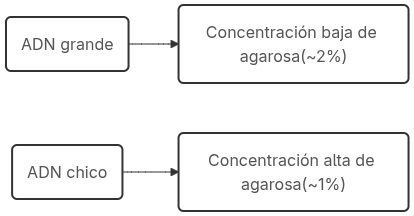
\includegraphics[width=\linewidth]{images/09_agarosa.png}
        \caption{Concentración de agarosa}
        \label{fig:agarosa-concentración}
    \end{subfigure}
    \hspace{0.1\textwidth}
    \begin{subfigure}{0.4\textwidth}
        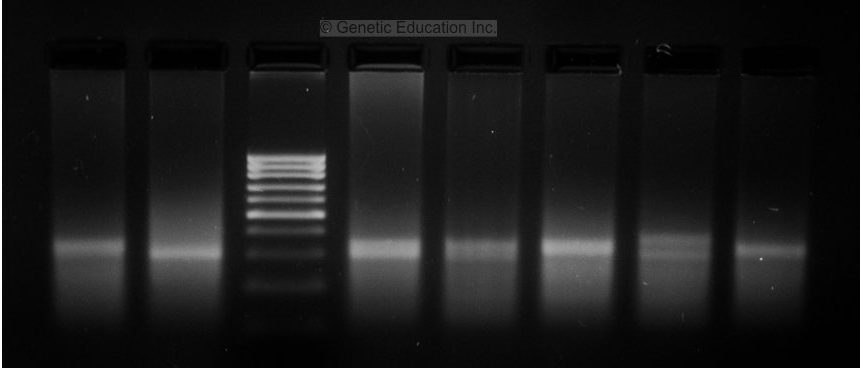
\includegraphics[width=\linewidth]{images/09_pcr-electro.jpg}
        \caption{Resultado}
        \label{fig:electro-gel}
    \end{subfigure}
    
    \caption{Electroforesis en gel después de una PCR}
    \label{fig:pcr-electro}
\end{figure}

\subsection{qPCR}

En el caso de una qPCR, el software del termociclador ya realiza una cuantificación de ADN, esto a través de la adición de colorantes antes de la realización de la PCR.

\subsubsection{SYBR Green}

Este es un colorante que se une a las cadenas dobles de ADN y que tiene cuerta fluorescencia, esto para hacerlas cuantificables por el equipo.

Este método \textbf{no es tan exacto}, esto porque que este colorante se une a todas las cadenas dobles de la muestra, no diferencia entre las originales y las generadas por la polimerasa. Para resolver esta incertidumbre se realiza una \textbf{curva de Melting}.

\begin{figure}[H]
    \centering
    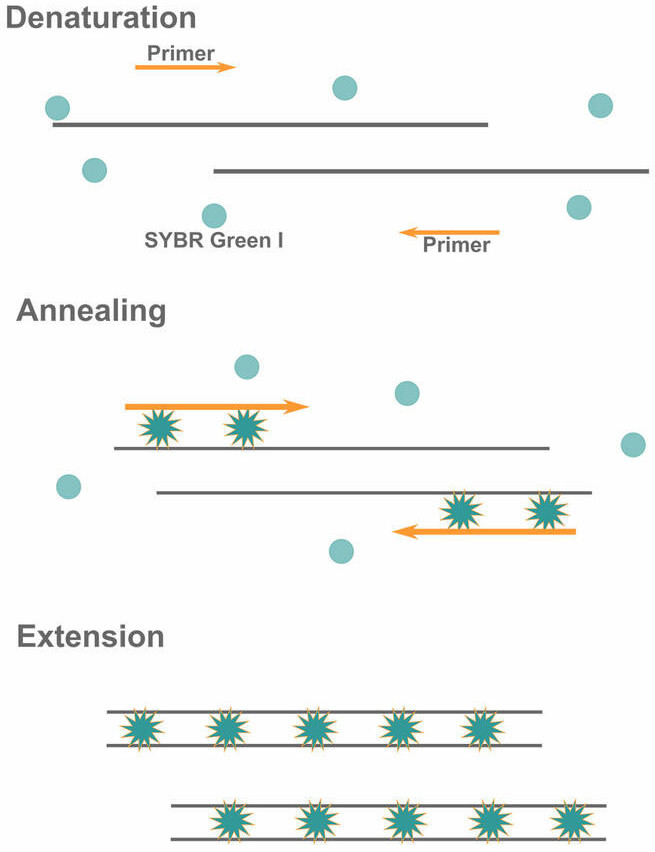
\includegraphics[width=0.65\linewidth]{images/09_sybr.jpg}
    \caption[Funcionamiento del colorante SYBR-Green]{Los círculos representan el SYBR-Green que \textbf{no emite luz}, mientras que las "estrellas" representa nel SYBR-Green que \textbf{ya emite luz}.}
    \label{fig:sybr-green}
\end{figure}

\subsubsection{Sonda Taq-Man}

Las sondas Taq-Man son moléculas que se componen de una cadena de nucleótidos que contiene un \textbf{fluoroforo (reportero)} en el \textbf{extremo 5'} y un \textbf{desactivador de fluorescencia (quencher)} en el \textbf{extremo 3'}.
Cuando se añaden las sondas a la muestra y las ADN se abren, las sondas se unen a zonas determinadas del ADN, pero por como están conformadas aún no pueden emitir luz que el termociclador pueda medir. Cuando inicia la PCR, la polimerasa avanza por la cadena de ADN y al llegar a la sonda Taq-Man la retira. Una vez liberada, los componentes de esta se separan y el reportero puede, ahora sí, emitir luz que puede ser medida por el termociclador.

Estas sondas, a comparación del SYBR Green, es \textbf{más específico}, pues hace que solo se midan las cadenas de ADN generadas, y no las originales de la muestra.

\begin{figure}[H]
    \centering
    
    \begin{subfigure}{0.4\textwidth}
        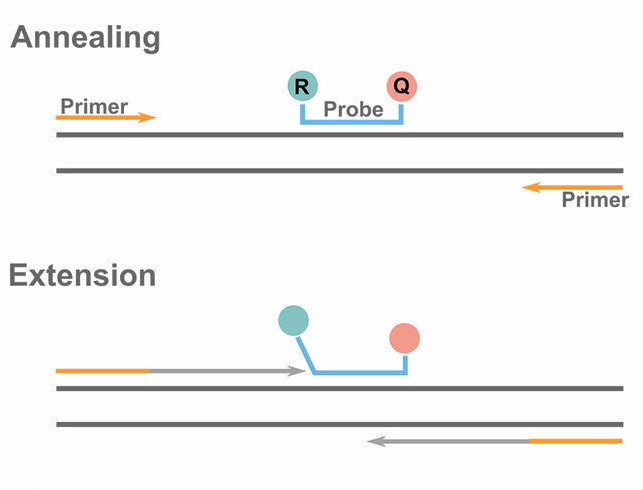
\includegraphics[width=\linewidth]{images/09_taqman-1.jpg}
        \caption{La sonda se une al ADN y el reportero no puede emitir luz. La polimerasa inicia la elongación.}
        \label{fig:taqman-1}
    \end{subfigure}
    
    \hspace{0.1\textwidth}
    
    \begin{subfigure}{0.4\textwidth}
        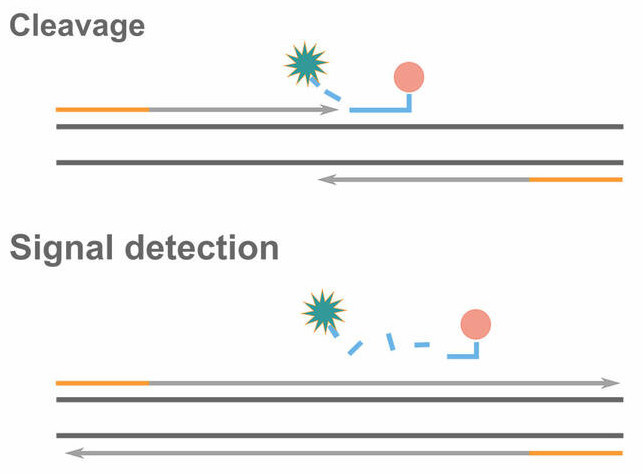
\includegraphics[width=\linewidth]{images/09_taqman-2.jpg}
        \caption{La polimerasa retira y deshace a la sonda. El reportero ahora puede emitir luz}
        \label{fig:taqman-2}
    \end{subfigure}
    
    \caption{Funcionamiento de las sondas TaqMan}
    \label{fig:taqman}
\end{figure}

\section{Recursos didácticos}

Se incluyen aquí algunos recursos que podrían ser de ayuda a conocer más sobre el tema.

\begin{figure*}[H]
    \centering
    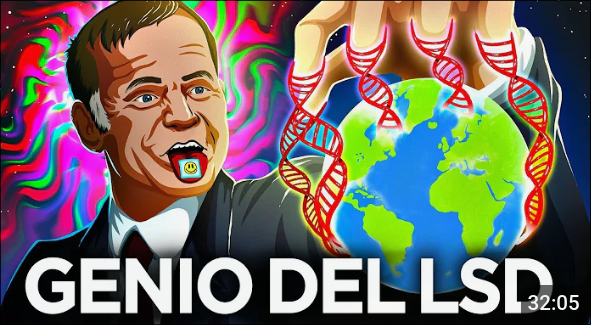
\includegraphics[width=0.5\textwidth]{images/09_veritasium.png}
    \caption{\href{https://youtu.be/uqngf-0pPC4?si=TOr9xlx6f40MSp0E}{El hombre que tomó LSD y cambió el mundo - Veritasium}}
    \label{fig:veritasium}
\end{figure*}

\begin{figure*}[H]
    \centering
    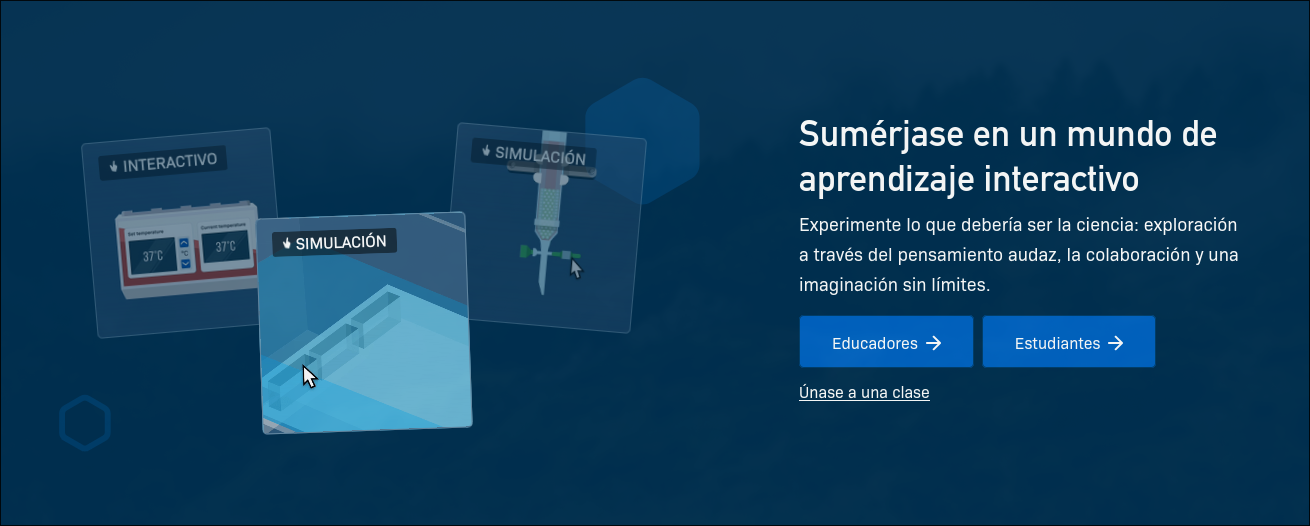
\includegraphics[width=0.5\textwidth]{images/09_labxchange.png}
    \caption{\href{https://www.labxchange.org/library}{Biblioteca general de LabXChange}}
    \label{fig:labxchange}
\end{figure*}

\begin{figure*}[H]
    \centering
    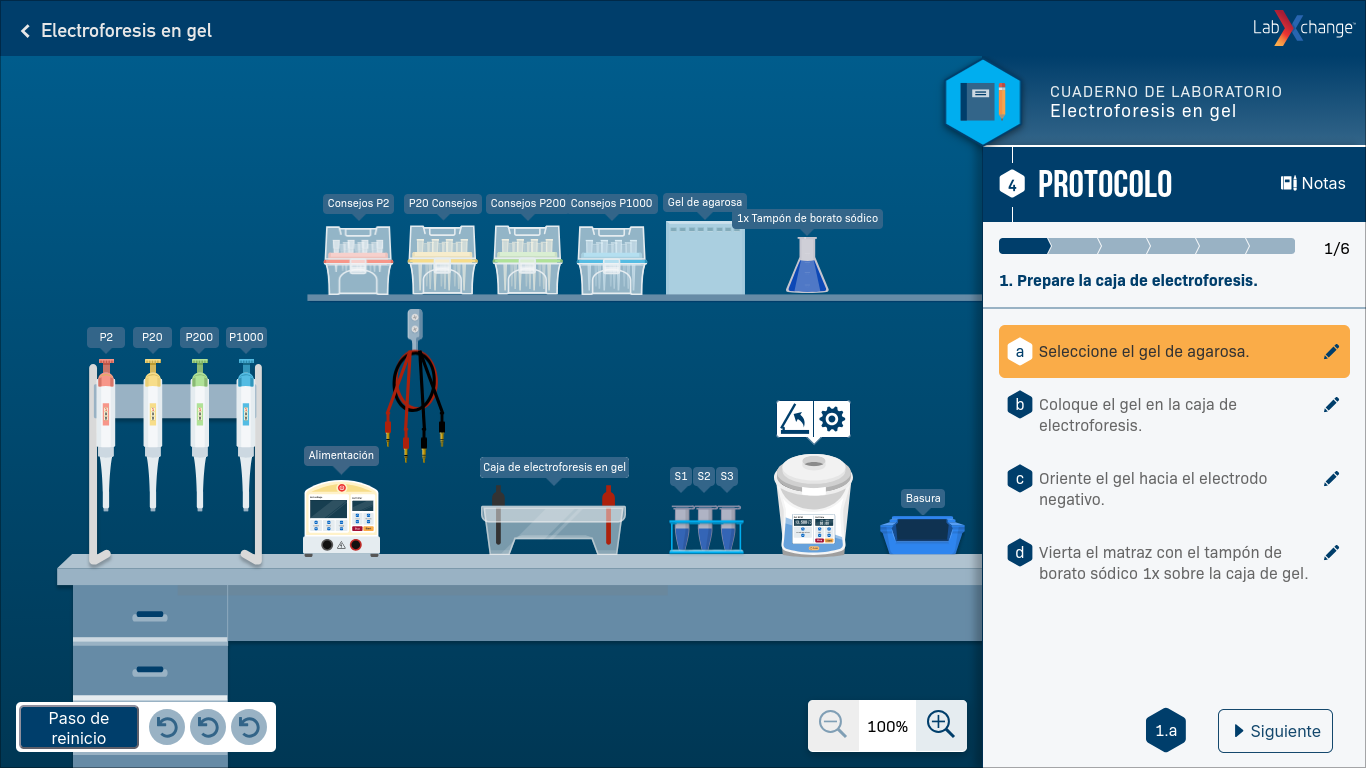
\includegraphics[width=0.5\textwidth]{images/09_lab-electro.png}
    \caption{\href{https://goo.su/uhRz17V}{Simulador de electroforesis}}
    \label{fig:labxchange}
\end{figure*}